\documentclass[12pt]{article}
\usepackage[pdftex]{graphicx}
\graphicspath{{pictures/}}
%\DeclareGraphicsExtensions{.pdf,.png,.jpg}
\usepackage{amsmath,amssymb,amsthm,latexsym,amsfonts}
\usepackage[utf8]{inputenc} % Включаем поддержку UTF8
\usepackage[T2A]{fontenc}
\usepackage{ucs}
\usepackage[russian]{babel}
\usepackage{amsthm}
\usepackage{graphicx}
\usepackage[unicode, pdftex]{hyperref}
\graphicspath{{pictures/}}
%\usepackage{indentfirst}
\DeclareGraphicsExtensions{.pdf,.png,.jpg,.eps}
\DeclareMathOperator*{\argmax}{argmax} % thin space, limits underneath in displays
\DeclareMathOperator*{\argmin}{argmin} % thin space, limits underneath in displays
\title{\LaTeX}
\date{}
\author{}

\usepackage{hyperref}
\usepackage{xcolor}
\definecolor{linkcolor}{HTML}{799B03} % цвет ссылок
\definecolor{urlcolor}{HTML}{799B03} % цвет гиперссылок
\hypersetup{pdfstartview=FitH,  linkcolor=linkcolor,urlcolor=urlcolor, colorlinks=true}


\begin{document}

\centerline{МОСКОВСКИЙ ГОСУДАРСТВЕННЫЙ УНИВЕРСИТЕТ}
\centerline{им. М.В.Ломоносова}
\centerline{ФАКУЛЬТЕТ ВЫЧИСЛИТЕЛЬНОЙ МАТЕМАТИКИ И КИБЕРНЕТИКИ}
\vfill
\centerline{КАФЕДРА МАТЕМАТИЧЕСКОЙ ФИЗИКИ}
%\centerline{\hfill\hrulefill\hrulefill\hfill}
\vfill
\vfill
\vfill
\large
\centerline{{Телепов} Александр Юрьевич}
\vfill
\Large
\begin{centering}
{\bf Реализация метода продолжения потенциала \\
для решения обратной задачи гравиметрии\\}
\end{centering}
\normalsize
\vfill
\centerline{Специальность 01.03.02~--- }
\centerline{прикладная математика и информатика}
\vfill
\centerline{Курсовая работа}
\vfill
\vfill
\begin{flushright}
Научный руководитель:\\
д.\,фм.\,н.~Дмитриев~В.\,И.
\end{flushright}
\vfill
\vfill
\centerline{Москва~--- 2019}
\clearpage

%\section
%{Аннотация}
%В данной работе исследуется возможность применения методов глубокого и машинного обучения для определения параметров источников гравитационного поля по нормальной составляющей ускорения свободного падения, измеренной на поверхности земли.
%Проведено сравнение классического подхода с нейросетевым подходом, а также с методом опроных векторов и  алгоритмом решающих деревьев.

\section
{Введение}
Гравиметрия — это нау­ка об из­ме­ре­нии ве­ли­чин, ха­рак­те­ри­зую­щих гравитационное по­ле Земли и других небесных тел. Гравиметрия рассматривает теории и методы измерения силы тяжести для решения различных задач геодезии, геофизики и других наук о Земле.\\
\newline
В разведочной геофизике гравиметрия используется для поиска и уточнения строения залежей полезных ископаемых, а также выявления предпосылок для их образования. Одно из основных геодезических приложений гравиметрии — построение моделей геоида. Точное знание геоида необходимо, в частности, в навигации — для пересчёта геодезических высот, непосредственно измеряемых GPS-приёмниками,
 а также в физической океанологии — для определения высот морской поверхности.\\
\newline
Особенностью обратных задач геофизики, в чатности — гравиметрии, является их некорректность. А именно обратная задача гравиметрии неустойчива и может иметь не единственное решение.
Некорректность обратной задачи гравиметрии связана с тем, что оператор ее прямой задачи является интегральным оператором первого рода.
Тоесть даже имея абсолютно точный обратный оператор можно получить сильно различающиеся решения при малых погрешностях в начальных данных, которые принципиально неизбежны в силу погрешности реальных измерений.\\
\newline
В данной работе исследуется возможность применения методов машинного обучения для определения параметров источников гравитационного поля по нормальной составляющей ускорения свободного падения, измеренной на поверхности земли.
\clearpage

\section
{Постановка задачи}

Основываясь на принципе суперпозиции, в прямой и обратной задачах гравиметрии используется только аномальное гравитационное поле:
\[U_a(M)=U(M)-U^N,\] где $U^N(M)$ - нормальный потенциал для некоторого среднего распределения плотности среды $\rho_N(M)$.\\
Далее всюду предполагается что мы имеем дело уже с аномальной плотностью, аномальным потенциалом и т.д.
\subsection
{Прямая задача}
По заданым области $V$ и аномальной плотности определить гравитационное поле на поверхности земли.\\
Решение дается в виде интеграла:\\
\[g(x,y)=\iiint\limits_{V_0}\frac{G\rho(M_0)cos\psi}{r^2}\,dv_0,\] где $G$ - гравитационная постоянная,\\
$\psi$ - угол между вертикалью и вектором $\vec{r} = \overrightarrow{MM_0}$,\\
 $cos\psi=\displaystyle\frac{z_0}{r}, r^2=(x-x_0)^2+(y-y_0)^2+z_0^2$.



\subsection
{Обратная задача}

По заданному на поверхности гравитационному полю $z=0$ определить форму области аномальной плотности $V$ и аномальную плотность $\rho(x,y,z)$.\\
\newline
По теореме Новикова если $V$ - звездна и $\rho = const$ в области $V$ то задача может иметь только 1 решение. В этом случае ищется поверхность $S$ - граница области $V$.\\
\newline
В данной работе рассматривается следущая модельная задача:\\
В заданной области на поверхности измерена нормальная составляющая ускорения свободного падения на равномерной сетке. \\
Требуется определить координаты $(x,y,z)$ всех источников гравитационного поля под поверхностью земли.\\
Считается, что источники имеют сферическую форму(за границей сферы поле точечного источника совпадает с полем сферы).\\
Заметим, что если мы умеем определять все параметры 1 любого источника, то мы можем решить задачу, последовательно вычитая поле найденного источника и снова находя параметры какого-либо из оставшихся источников.

\section
{Метод продолжения гравитационного поля}

Алгоритмы продолжения гравитационного поля вглубь земли используются для уменьшения влияния совокупности источников на создаваемое поле в окрестности отдельно взятого тела.\\
\newline
Рассмотрим поведение карт напряженности гравитационного при увеличении глубины их построения $z$.
При стремлении $z$ к $z_{i}$ - координате залегания $i$-го тела $g(x_i,y_i)$ будет стремиться к плюс бесконечности и определяться практически характеристиками только $i$-го тела.
Следовательно если мы умеем продолжать гравитационное поле, то сможем легко определить координаты $(x,y)$ всех источников.\\
\newline
Таким образом при продолжении гравитационного поля вглубь земли лучше проявляются характеристики источников поля.\\

Рассмотрим поведение $f_{p}(h)=\displaystyle{\frac{{\partial}g(h,p)}{{\partial}h}}(h)$.
\[g(h,p)=\frac{GM}{h^2+p^2}\]
\[f_p(h)=\frac{-2GMh}{(p^2+h^2)^2}\]
$f_p(h)$ имеет единственный минимум в точке $\displaystyle{h_{*}=\frac{p}{\sqrt{3}}}$, равный $\displaystyle\frac{-MG}{8h_{*}}$.
Умея продолжать нпаряженность гравитационного поля мы можем численно считать производную по $h$ и сторить ее график. По нему мы можем найти $h_{*}$
и $f_p(h_{*})$ . Отсюда находится $M=\displaystyle\frac{8f_p(h_{*})h_{*}}{G}$.

Найдем \[I = \iint\limits_{S:x^2+y^2{\leq}p_0^2} g(x,y) \,dxdy = \iint\limits_{S:x^2+y^2{\leq}p_0^2} g(h,p) p\,dpd{\varphi} \].
 \[I = \iint\limits_{S:x^2+y^2{\leq}p_0^2} g(h,p) p\,dpd{\varphi} = \frac{1}{2}GMh{\int\limits_{0}^{2\pi}\,d{\varphi}}{\int\limits_{0}^{p_0}\frac{2p}{(h^2+p^2)^{\frac{3}{2}}}\,dp}=\]
\[=2{\pi}GM\left(\frac{1}{h}-\frac{1}{\sqrt{p_0^2+h^2}} \right)\]

Обозначим $$f_c(x)=1-\frac{x}{\sqrt{c^2+x^2}}$$

Тогда \[h = f_{p_0}^{-1}\left({\frac{I}{-4{\pi}GM}} \right)\].
\[f_c^{-1}(x)={\frac{c(1-x^2)}{\sqrt{1-(1-x^2)^2}}}\]
\newline
Для решения обратной задачи предлагается использовать метод продолжения гравитационного потенциала \cite{dmitriev2012iterative1786867}.\\
\newline
Пусть ${\Delta}U=0$, $z{\geqslant}h$,
 $x,y {\in} \mathbb{ R}$\\
	$U{\longrightarrow}0$ регулярно, 
$r{\longrightarrow}{\infty}$\\
Возьмем функцию Грина в виде \[G(M,M_0)=\frac{1}{\sqrt{(x-x_0)^2+(y-y_0)^2+(z-z_0)^2}}+\frac{1}{\sqrt{(x-x_0)^2+(y-y_0)^2+(z-z_0-2h)^2}}\]
Учтем, что $\displaystyle\frac{{\partial}G(x_0,y_0,z_0)}{{\partial}z_0}{\Bigr|_{{z}=h}}=0$ и применим интегральную формулу Грина:\\
\[V(x,y,z)=\frac{1}{4\pi}\iint\limits_{\Sigma}\left({G\frac{{\partial}V}{{\partial}n} - V\frac{{\partial}G}{{\partial}n}}\right)\,d{\sigma} - \frac{1}{4\pi}\iiint\limits_{\Omega}G{\Delta}V\,d{\Omega}\]
Если $V$ - гармоническая, то:
\[V(x,y,z)=\frac{1}{4\pi}\iint\limits_{{-\infty}{-\infty}}^{{+\infty}{+\infty}}G(M,M_0){\Bigr|_{{z_0}=h}}\frac{{\partial}V(x_0,y_0,z_0)}{{\partial}z_0}{\Bigr|_{{z_0}=h}}\,dx_0dy_0\]\\

Так как $$G(M,M_0){\Bigr|_{{z_0}=h}}=\frac{2}{\sqrt{(x-x_0)^2+(y-y_0)^2+(z-h)^2}}$$ \\

получим \\
\[V(x,y,z)=\frac{1}{2\pi}\iint\limits_{{-\infty}{-\infty}}^{{+\infty}{+\infty}}\frac{{\partial}V(x_0,y_0,z_0)}{{\partial}z_0}{\Bigr|_{{z_0}=h}\frac{1}{\sqrt{(x-x_0)^2+(y-y_0)^2+(z-h)^2}}}\,dx_0dy_0\]

Заметим, что \[{\Delta}U(M)=-4{\pi}{\rho}(M),\] 
 \[\frac{{\partial}U}{{\partial}z}=g_z(x,y,z)\] \\
Записав формулу для $U(x,y,z)$ в области, где отстутвуют источники($\rho(M_0)=0$) и продифференцировав по $z$ получим:
\[g_z(x,y,z)=\frac{1}{2\pi}\iint\limits_{{-\infty}{-\infty}}^{{+\infty}{+\infty}}\frac{g_z(x_0,y_0,h)(h-z)}{((x-x_0)^2+(y-y_0)^2+(h-z)^2)^{\frac{3}{2}}} \,dx_0dy_0\]
Это - интегральное уравнение первого рода для напряженности на глубине $z=h$ с $\delta$-образным ядром. Решение этого уравнения является некорректной задачей.\\
В \cite{dmitriev2012iterative1786867} был предложен итерационный метод решения данного интегрального уравнения.\\
Перепишем уравнение в  виде \[g(x,y,h)+\frac{h}{\pi}\iint\limits_{{-\infty}{-\infty}}^{{+\infty}{+\infty}}\frac{g(x_0,y_0,h)-g(x,y,h)}{((x-x_0)^2+(y-y_0)^2+(h-z)^2)^{\frac{3}{2}}} \,dx_0dy_0=g(x,y,0)\]
Итерационный процесс записывается следущим образом:
\[g_n(x,y,h)=g_{n-1}+g(x,y,0)-\frac{h}{\pi}\iint\limits_{{-\infty}{-\infty}}^{{+\infty}{+\infty}}\frac{g_{n-1}(x_0,y_0,h)}{((x-x_0)^2+(y-y_0)^2+(h-z)^2)^{\frac{3}{2}}} \,dx_0dy_0\]

\section
{Численные эксперименты}

Для сравнения методов планируется взять некоторое количество случайно сгенерированных полей при различных уровнях зашумлености(к исходному правильно вычисленному полю прибавляется случайный шум, взятый из некоторого фиксированного распределения).\\
Результаты курсовой работы будут представлены в виде графиков точности определения параметров источников гравитационного поля от уровня шума в начальных данных для предложенных методов решения обратной задачи.\\
Также критериями качества метода будет являться скорость работы, а также возможность и эффективность параллельной реализации.


В главе 2.1 был описан итерационный метод решения интегрального уравнения с $\delta$-образным ядром.\\
 Считая $U_z(x,y)$ равной 0 всюду вне $$S = \left[{-N, N} \right] \times \left[{-M, M} \right] $$ 
и постоянной в областях $$x \in \left[{\left({n-\frac{1}{2}}\right)h_x,\left({n+\frac{1}{2}}\right)h_x} \right] , y \in \left[\left({m-\frac{1}{2}}\right)h_y,\left({m+\frac{1}{2}}\right)h_y \right] $$ 

Формула из главы 2.1 преобразуется в:\\
\[U_{nm}^s=U_{nm}^{s-1}-\sum_{i=-N}^N{\sum_{j=-M}^M a_{ij}^{nm}U_{ij}^{s-1}}\]

$$n \in \left[{-N,N} \right] , m \in \left[{-M, M} \right] $$\\
$$x_n=nh_x, y_m=mh_y$$
%\small
\[a_{ij}^{nm} = \varphi(x_i-x_n+\frac{h_x}{2},y_j-y_m+\frac{h_y}{2}) + \varphi(x_i-x_n-\frac{h_x}{2},y_j-y_m-\frac{h_y}{2}) -\] \[- \varphi(x_i-x_n-\frac{h_x}{2},y_j-y_m+\frac{h_y}{2}) - \varphi(x_i-x_n+\frac{h_x}{2},y_j-y_m-\frac{h_y}{2})\]
%\normalsize

\[\varphi(x,y)=\frac{1}{2\pi}arctg\left({\frac{xy}{z\sqrt{x^2+y^2+z^2}}}\right)\]
\newline
При последовательном увелечении глубины алгоритм будет уточнять глубину залегания ближайщего источника, т.к влияние остальных тел будет уменьшаться.
После пересечения глубины залегания источника алгоритм будет искать такой источник под «перескоченным», которой будет давать мало отличающеся на поверхности поле. Мощность и глубина залегания такого источника источника увеличатся - это мы и возьмем за критерий останова.

Метод продолжения потенциала был реализован на языке python с использованием библиотек pytorch, numpy, matplotlib и plotly. Все исходные коды и резльтаты работы можно найти в репозитории \href{https://github.com/AlexandrTelepov/diploma}{https://github.com/AlexandrTelepov/diploma}.
Численные эксперементы проводились над полями сгенерированными по формуле (1), все операции проводились над числами с двойной точностью.
Разное колличество итераций.

%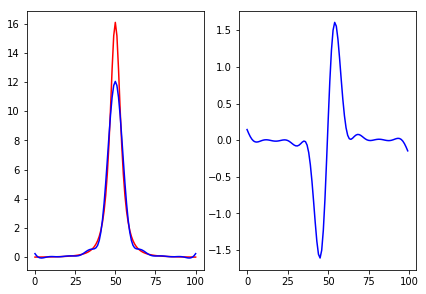
\includegraphics{picture1}
\begin{figure}[h]
\begin{minipage}[h]{0.49\linewidth}
\center{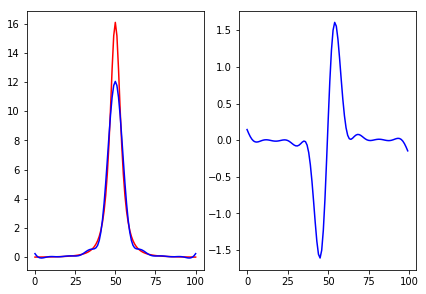
\includegraphics[width=0.5\linewidth]{picture1}}
\caption{Описание}
\label{fig:image}
\end{minipage}
\hfill
\begin{minipage}[h]{0.49\linewidth}
\center{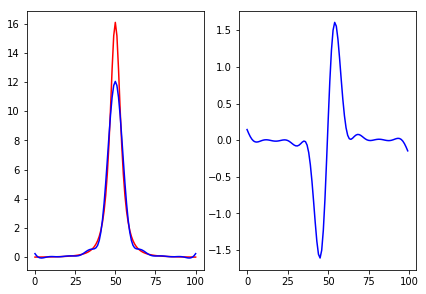
\includegraphics[width=0.5\linewidth]{picture1}}
\caption{Описание}
\label{fig:image}
\end{minipage}
\end{figure}

\section
{Заключение}
В данной работе реализован метод продолжения потенциала для решения обратной задачи гравиметрии. Были проведены численные эксперименты с различными конфигурациями источников гравитационного поля. Результаты показывают эффективность предложенного метода.
\clearpage

\bibliographystyle{utf8gost705u}
\bibliography{biblio}
\end{document}